\documentclass[conference]{IEEEtran}
\usepackage[utf8]{inputenc}
\usepackage{graphicx}
\usepackage{amsmath}
\usepackage{cite}
\usepackage{url}
\usepackage[none]{hyphenat}
\usepackage{float}
\usepackage{tikz}
\usepackage{algorithm}
\usepackage{algpseudocode}
\usepackage{microtype}
\usepackage{ragged2e}
\usepackage[colorlinks=true,citecolor=black,linkcolor=black,urlcolor=black]{hyperref}

\tolerance=1%
\emergencystretch=\maxdimen%
\hyphenpenalty=10000%
\exhyphenpenalty=100%

\usetikzlibrary{arrows.meta, positioning, shapes.geometric}

\title{Anti-Plagiarism System for Exam Monitoring}

\author{
    \IEEEauthorblockN{Valentin Pletea-Marinescu}
    \IEEEauthorblockA{
        \textit{National University of Science and Technology }\\
        \textit{POLITEHNICA Bucharest} \\
        Email: \texttt{valentin.pletea@stud.acs.upb.ro}
    }
    \and
    \IEEEauthorblockN{Ge Su}
    \IEEEauthorblockA{
        \textit{Zhejiang University}\\
        Email: \texttt{suge@zju.edu.cn}
    }
    \and
    \IEEEauthorblockN{Ștefan-Dan Ciocîrlan}
    \IEEEauthorblockA{
        \textit{National University of Science and Technology }\\
        \textit{POLITEHNICA Bucharest} \\
        Email: \texttt{stefan\_dan.ciocirlan@upb.ro}
    }
    \and
    \IEEEauthorblockN{Ștefan-Alexandru Mocanu}
    \IEEEauthorblockA{
        \textit{National University of Science and Technology }\\
        \textit{POLITEHNICA Bucharest} \\
        Email: \texttt{stefan.mocanu@upb.ro}
    }
}

\begin{document}

\maketitle

\begin{abstract}
Academic integrity represents a fundamental challenge in modern education systems, 
with plagiarism rates increasing globally across all educational levels. Traditional 
exam monitoring approaches rely primarily on screen surveillance and human oversight, 
creating significant vulnerabilities in detecting sophisticated cheating behaviors 
during online and remote examinations.
This research develops a comprehensive anti-plagiarism monitoring system using 
deep learning and computer vision technologies to address these limitations. 
The system integrates gaze tracking algorithms with YOLO-based object detection 
models through a modular software architecture. Facial landmark detection enables 
precise gaze direction analysis, while specialized convolutional neural networks 
identify unauthorized objects and suspicious materials in the examination environment. 
These two complementary approaches work together to provide comprehensive monitoring 
coverage: gaze analysis detects abnormal visual attention patterns that may indicate 
unauthorized assistance seeking, while object detection identifies physical cheating 
aids such as smartphones and smartwatches.
Experimental testing demonstrates effective operation on CPU-based 
systems, identifying suspicious gaze patterns, abnormal behaviors, 
and unauthorized objects while maintaining real-time performance. The system provides 
comprehensive exam monitoring capabilities suitable for educational institutions, enabling 
widespread deployment using standard computing hardware without requiring specialized equipment.
\end{abstract}

\begin{IEEEkeywords}
Academic integrity, Educational technology, Computer vision, Gaze tracking, Object detection, Real-time systems, Machine learning, Convolutional neural networks, Image processing, Kalman Filters
\end{IEEEkeywords}

% === INTRODUCTION ===
\section{Introduction}
Academic integrity remains a core educational challenge. Recent studies\cite{abbas2022review,alsabhan2023,newton2024,noorbehbahani2022} highlight increased exam fraud during post-pandemic online learning. Traditional tools fail to detect physical cheating like gaze aversion or unauthorized devices. 
Research demonstrates that academic dishonesty affects educational quality, credibility, and institutional reputation\cite{zhao2022,reedy2021}. Recent statistics reveal concerning trends, with some regions reporting plagiarism detection rates exceeding 26\% of submitted academic works\cite{noorbehbahani2022}.

Traditional examination monitoring approaches present significant limitations in detecting sophisticated cheating behaviors, particularly in remote and hybrid learning contexts\cite{nigam2021}. These approaches rely on manual supervision and screen-based surveillance, failing to detect physical cheating behaviors such as unauthorized device usage or suspicious gaze patterns, creating vulnerabilities in examination integrity\cite{ahmad2021}.

While machine learning solutions exist for plagiarism detection\cite{kamalov2021,chen2023deep}, most require computational resources including GPU acceleration, making them inaccessible to many educational institutions with limited hardware infrastructure.

Recent advances in computer vision and artificial intelligence have opened possibilities for automated monitoring systems. Studies have demonstrated the effectiveness of facial detection algorithms in real-time applications\cite{markerless2021,artfacepoints2022,aung2022real}. Research in eye-tracking technology has shown promising results for behavioral analysis in educational contexts\cite{jarodzka2021,akinyelu2021cnn,frontiersgaze2024}. 

Furthermore, object detection technologies, particularly YOLO architectures, have revolutionized real-time identification capabilities\cite{yi2023small}. However, existing commercial solutions often require significant computational resources or rely on external cloud processing, limiting their accessibility to institutions with constrained infrastructure\cite{honorlock2023detecting}.

This paper presents an anti-plagiarism monitoring system that operates on standard CPU-based hardware, requiring minimal computational resources while maintaining high detection accuracy. The system demonstrates real-time performance on hardware configurations, including Intel i5 7th generation processors, making monitoring technology accessible to institutions regardless of their technical infrastructure limitations.

The paper is organized as follows: Section II discusses related work in computer vision 
fundamentals and educational technology integration. Section III presents the overall 
system framework and methodology. Section IV describes the technical details of the 
implementation. Section V evaluates the system's performance and presents experimental 
results. Section VI provides insights from the discussion, and Section VII concludes 
our work and outlines directions for future research.

% === BACKGROUND ===
\section{Background}

\subsection{Facial Landmark Detection and Gaze Tracking}
Facial landmark detection is fundamental for behavioral monitoring in exam environments. Modern deep learning models such as MediaPipe Face Mesh\cite{jakhete2024comprehensive} can extract 468 real-time 3D facial landmarks, far surpassing traditional 68-point methods\cite{markerless2021,artfacepoints2022}. This high granularity enables precise localization of eyes, iris, and facial contours, supporting robust gaze estimation even under variable lighting or head movement.

Gaze tracking leverages these landmarks to compute gaze direction vectors, identifying deviations from normal behavior (e.g., repeated side glances or downward gaze). To reduce noise and stabilize estimates in the presence of rapid movement or occlusion, advanced Kalman filters are used\cite{aung2022real,jeong2014kalman,li2020hksiamfc}. These filters model eye movement as a dynamic process, filtering outliers and ensuring smooth, continuous gaze tracking.

\subsection{YOLO and Object Detection}
Object detection is essential for identifying unauthorized devices (phones, smartwatches) in the exam environment. YOLO (You Only Look Once) algorithms, now at v8 \cite{yi2023small}, provide fast and accurate detection of small objects in video frames, enabling real-time processing on standard hardware.

YOLOv8 uses optimized convolutional neural network architectures for speed and accuracy, with significant reductions in parameters and computational cost compared to earlier versions. These models can be trained on custom datasets to recognize exam-specific devices, maintaining low false alarm rates even under challenging lighting or background conditions.

\subsection{AI-Based Monitoring}
Modern automated anti-plagiarism solutions use artificial intelligence to detect non-compliant behaviors during online exams. Recent systems\cite{kaddoura2022,abbas2022review,alsabhan2023,nigam2021,ahmad2021} employ convolutional neural networks (CNNs) for face and object recognition, as well as LSTM networks for temporal behavior analysis (e.g., gaze or repetitive movements over time).

A major advantage of the presented approach is fully offline processing, with no dependence on cloud or external servers, ensuring data privacy and reducing costs. The system operates efficiently on standard CPU hardware, making it accessible to educational institutions with limited resources.

By combining gaze detection, object identification, and temporal analysis, the system provides comprehensive coverage of potential cheating behaviors, overcoming the limitations of traditional screen-capture or human-only supervision.

% === SYSTEM ARCHITECTURE AND METHODOLOGY ===
\section{System Architecture and Methodology}

\subsection{Modular System Design}

The anti-plagiarism system uses a modular architecture with five components: 
facial detection, gaze analysis, object detection, violation monitoring, and 
report generation. The facial detection module identifies faces and extracts 
468-point landmarks (via MediaPipe Face Mesh). The gaze analysis module 
uses these landmarks to compute the candidate's gaze direction, flagging 
abnormal looking-away behavior. The object detection module employs 
YOLOv8 models to detect unauthorized devices (e.g., phones, watches) in 
the scene. The violation monitoring module fuses information from the gaze 
and object detectors to identify exam rule violations. Finally, the report 
generation module logs the session results and creates a monitoring report.

\subsection{Gaze Analysis Subsystem}
This subsystem processes MediaPipe Face Mesh landmark data to determine 
the candidate’s gaze direction. We calculate horizontal and vertical gaze 
ratios based on key facial landmarks and apply Kalman filtering to smooth 
the results. Head orientation is compensated for using additional landmarks 
(e.g., chin, forehead). The module classifies gaze as left, right, center, or 
down, enabling detection of abnormal eye movements relative to normal 
exam behavior.

\subsection{Object Detection Framework}

The object detection component utilizes specialized recognition models to identify 
unauthorized devices within the examination environment. The framework employs separate 
detection pathways for different device categories, enabling optimized recognition 
thresholds and reduced classification errors.

The architecture supports real-time processing through intelligent frame selection 
strategies that balance detection accuracy with computational efficiency. The framework 
processes video streams at optimized intervals while maintaining continuous monitoring 
capabilities for immediate violation detection.

\subsection{Integration and Performance}

The system architecture implements a publisher-subscriber communication pattern that 
enables asynchronous coordination between detection modules and the central violation 
monitoring system. This architectural approach ensures system responsiveness while 
accommodating varying processing requirements across different detection algorithms.

The violation monitoring module serves as the central coordination point, aggregating 
detection results from multiple independent sources. The module applies temporal analysis 
to reduce false positive detections caused by brief, natural movements while maintaining 
sensitivity to genuine violations.

Modules communicate via PyQt5 signals, enabling asynchronous processing and a responsive UI. In real-time tests, CPU utilization peaked at 27\%, allowing for multi-hour continuous monitoring.

\subsection{System Architecture Diagrams and Operational Analysis}

To illustrate the system structure and operation, two complementary UML diagrams have 
been developed: the activity diagram and sequence diagram. These representations offer 
different perspectives on the architecture, from operational flow to temporal component 
interactions.

\subsubsection{Activity Diagram and Operational Flow}

The activity diagram presents the comprehensive operational flow of the anti-plagiarism 
system, illustrating decision points and parallel processing capabilities that distinguish 
this implementation from conventional monitoring solutions.

\begin{figure}[H]
    \centering
    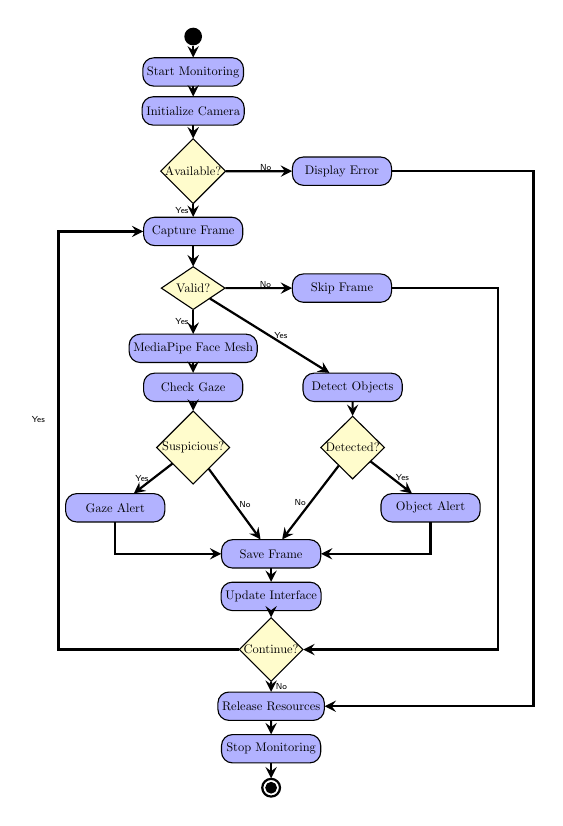
\begin{tikzpicture}[
        scale=0.45,
        transform shape,
        node distance=1.0cm,
        start/.style={circle, fill=black, minimum width=0.5cm},
        end/.style={circle, draw=black, thick, fill=white, minimum width=0.5cm},
        process/.style={rectangle, draw=black, fill=blue!30, minimum width=2.8cm, 
                        minimum height=0.8cm, text centered, rounded corners},
        decision/.style={diamond, draw=black, fill=yellow!20, text centered, 
                        minimum width=1.8cm, minimum height=0.7cm, inner sep=0pt},
        arrow/.style={thick, ->, >=stealth}
    ]
        \node[start] (initpoint) {};
        \node[process, below of=initpoint] (start) {Start Monitoring};
        \node[process, below of=start, yshift=-0.1cm] (init) {Initialize Camera};
        
        \node[decision, below of=init, yshift=-0.7cm] (cameracheck) {Available?};
        \node[process, right of=cameracheck, xshift=3.2cm] (errorcamera) {Display Error};
        
        \node[process, below of=cameracheck, yshift=-0.7cm] (capture) {Capture Frame};
        \node[decision, below of=capture, yshift=-0.6cm] (framecheck) {Valid?};
        \node[process, right of=framecheck, xshift=3.2cm] (errorframe) {Skip Frame};
        
        \node[process, below of=framecheck, yshift=-0.7cm] (face) {MediaPipe Face Mesh};
        
        \node[process, below of=face, yshift=-0.1cm] (gazecheck) {Check Gaze};
        \node[process, right of=gazecheck, xshift=3.5cm] (objectcheck) {Detect Objects};
        
        \node[decision, below of=gazecheck, yshift=-0.7cm] (gazeviolation) {Suspicious?};
        \node[decision, below of=objectcheck, yshift=-0.7cm] (objectviolation) {Detected?};
        
        \node[process, below of=gazeviolation, xshift=-2.2cm, yshift=-0.7cm] (gazealert) {Gaze Alert};
        \node[process, below of=objectviolation, xshift=2.2cm, yshift=-0.7cm] (objectalert) {Object Alert};
        
        \node[process, below of=gazeviolation, yshift=-2.0cm, xshift = 2.2cm] (save) {Save Frame};
        \node[process, below of=save, yshift = -0.2cm] (update) {Update Interface};
        \node[decision, below of=update, yshift=-0.5cm] (continue) {Continue?};
        \node[process, below of=continue, yshift=-0.6cm] (cleanup) {Release Resources};
        \node[process, below of=cleanup, yshift=-0.2cm] (stop) {Stop Monitoring};
        
        \node[end, below of=stop, yshift=-0.1cm] (endnode) {};
        \filldraw[black] (endnode.center) circle (0.15cm);
        
        \draw[arrow] (initpoint) -- (start);
        \draw[arrow] (start) -- (init);
        \draw[arrow] (init) -- (cameracheck);
        
        \draw[arrow] (cameracheck) -- node[right, xshift=-0.1cm, yshift=+0.1cm, font=\sffamily\scriptsize] {No} (errorcamera);
        \draw[arrow] (cameracheck) -- node[left, font=\sffamily\scriptsize] {Yes} (capture);
        \draw[arrow] (errorcamera.east) -- ++(4.0,0) |- (cleanup.east);
        
        \draw[arrow] (capture) -- (framecheck);
        \draw[arrow] (framecheck) -- node[right, xshift=-0.1cm, yshift=+0.1cm, font=\sffamily\scriptsize] {No} (errorframe);
        \draw[arrow] (framecheck) -- node[left, font=\sffamily\scriptsize] {Yes} (face);
        \draw[arrow] (framecheck) -- node[right, font=\sffamily\scriptsize] {Yes} (objectcheck);
        \draw[arrow] (errorframe.east) -- ++(3.0,0) |- (continue.east);
        
        \draw[arrow] (face) -- (gazecheck);  
        
        \draw[arrow] (gazecheck) -- (gazeviolation);
        \draw[arrow] (objectcheck) -- (objectviolation);
        
        \draw[arrow] (gazeviolation) -- node[left, font=\sffamily\scriptsize] {Yes} (gazealert);
        \draw[arrow] (objectviolation) -- node[right, font=\sffamily\scriptsize] {Yes} (objectalert);
        
        \draw[arrow] (gazeviolation) -- node[right, font=\sffamily\scriptsize] {No} (save);
        \draw[arrow] (objectviolation) --node[left, font=\sffamily\scriptsize] {No} (save);
        \draw[arrow] (gazealert) |- (save);
        \draw[arrow] (objectalert) |- (save);
        
        \draw[arrow] (save) -- (update);
        \draw[arrow] (update) -- (continue);
        \draw[arrow] (continue) -- node[right, font=\sffamily\scriptsize] {No} (cleanup);
        \draw[arrow] (cleanup) -- (stop);
        \draw[arrow] (stop) -- (endnode);
        
        \draw[arrow] (continue) -- node[left, xshift=-2.8cm, yshift=6.5cm, font=\sffamily\scriptsize] {Yes} ++(-6,0) |- (capture.west);
    \end{tikzpicture}
    \caption{Activity diagram of the anti-plagiarism system}
\end{figure}

The activity diagram demonstrates the operational flow beginning with system 
initialization through Start Monitoring, triggered when users activate monitoring 
through the graphical interface. The Initialize Camera process configures capture 
parameters and establishes webcam connectivity, implementing error handling through 
the Available decision point.

\textbf{Runtime Camera Health Monitoring:} The system implementation incorporates 
continuous camera health monitoring within the Capture Frame process. When frame 
capture fails repeatedly (indicating camera loss), the system triggers an emergency 
shutdown sequence that bypasses normal processing and routes directly to cleanup 
procedures. This ensures graceful termination rather than application crashes when 
hardware becomes unavailable during examination sessions.

\textbf{Parallel Processing Architecture:} The system's innovation emerges after 
frame validation, where processing branches into two independent parallel streams:

\textit{Behavioral Analysis Stream:} Executes MediaPipe Face Mesh with 468-point 
facial landmark detection, followed by Check Gaze implementing the horizontal and 
vertical ratio algorithms for gaze direction analysis. The core behavioral monitoring 
focuses specifically on gaze pattern analysis to detect visual attention directed 
away from examination materials.

\textit{Object Detection Stream:} Processes Detect Objects using dual YOLOv8 models 
for mobile phones and smartwatches. The Detected decision applies confidence thresholds 
(0.65 for both), producing Object Alert for unauthorized devices.

\textbf{Robust Error Handling:} Update Interface refreshes the display through PyQt5 
signals, providing real-time feedback to supervisors including camera health status 
indicators. The monitoring loop returns to Capture Frame for sustained operation or 
advances to cleanup procedures when termination conditions are met, ensuring proper 
resource management under all operational scenarios.

\subsubsection{Sequence Diagram Analysis}

The sequence diagram reveals temporal interactions between system components, illustrating 
message passing and activation patterns critical for real-time operation with MediaPipe 
Face Mesh integration.

\begin{figure}[H]
    \centering
    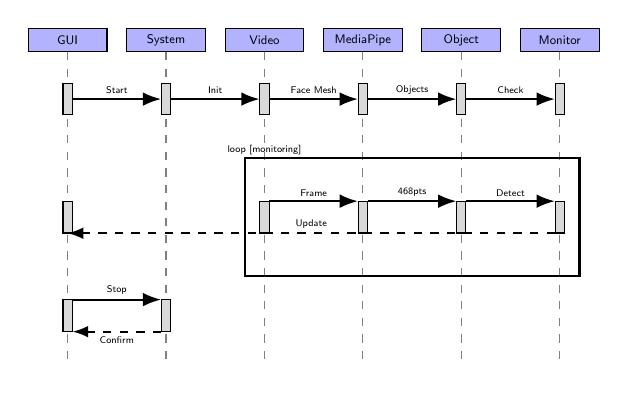
\begin{tikzpicture}[
        scale=0.5,
        transform shape,
        participant/.style={rectangle, draw=black, fill=blue!30, text centered, minimum width=2.0cm, minimum height=0.6cm, font=\sffamily\small},
        activation/.style={rectangle, draw=black, fill=gray!30, minimum width=0.2cm},
        lifeline/.style={dashed},
        message/.style={-{Latex}, thick},
        return/.style={-{Latex[length=2mm]}, dashed, thick},
    ]
        \node[participant] (gui) at (0,0) {GUI};
        \node[participant] (sistem) at (2.5,0) {System};
        \node[participant] (video) at (5,0) {Video};
        \node[participant] (mediapipe) at (7.5,0) {MediaPipe};
        \node[participant] (object) at (10,0) {Object};
        \node[participant] (violation) at (12.5,0) {Monitor};
        
        \draw[lifeline, gray] (gui.south) -- +(0,-8);
        \draw[lifeline, gray] (sistem.south) -- +(0,-8);
        \draw[lifeline, gray] (video.south) -- +(0,-8);
        \draw[lifeline, gray] (mediapipe.south) -- +(0,-8);
        \draw[lifeline, gray] (object.south) -- +(0,-8);
        \draw[lifeline, gray] (violation.south) -- +(0,-8);
        
        \node[activation] (gui_act1) at (0,-1.5) [minimum height=0.8cm] {};
        \node[activation] (sistem_act1) at (2.5,-1.5) [minimum height=0.8cm] {};
        \node[activation] (video_act1) at (5,-1.5) [minimum height=0.8cm] {};
        \node[activation] (mediapipe_act1) at (7.5,-1.5) [minimum height=0.8cm] {};
        \node[activation] (object_act1) at (10,-1.5) [minimum height=0.8cm] {};
        \node[activation] (violation_act1) at (12.5,-1.5) [minimum height=0.8cm] {};
        
        \draw[message] (gui_act1) -- node[above, font=\sffamily\scriptsize] {Start} (sistem_act1);
        \draw[message] (sistem_act1) -- node[above, font=\sffamily\scriptsize] {Init} (video_act1);
        \draw[message] (video_act1) -- node[above, font=\sffamily\scriptsize] {Face Mesh} (mediapipe_act1);
        \draw[message] (mediapipe_act1) -- node[above, font=\sffamily\scriptsize] {Objects} (object_act1);
        \draw[message] (object_act1) -- node[above, font=\sffamily\scriptsize] {Check} (violation_act1);
        
        \draw[thick] (4.5,-3) rectangle (13,-6);
        \node[font=\sffamily\scriptsize] at (5,-2.8) {loop [monitoring]};
        
        \node[activation] (video_act2) at (5,-4.5) [minimum height=0.8cm] {};
        \node[activation] (mediapipe_act2) at (7.5,-4.5) [minimum height=0.8cm] {};
        \node[activation] (object_act2) at (10,-4.5) [minimum height=0.8cm] {};
        \node[activation] (violation_act2) at (12.5,-4.5) [minimum height=0.8cm] {};
        \node[activation] (gui_act2) at (0,-4.5) [minimum height=0.8cm] {};

        \draw[message] (video_act2.north east) -- node[above, font=\sffamily\scriptsize] {Frame} (mediapipe_act2.north west);
        \draw[message] (mediapipe_act2.north east) -- node[above, font=\sffamily\scriptsize] {468pts} (object_act2.north west);
        \draw[message] (object_act2.north east) -- node[above, font=\sffamily\scriptsize] {Detect} (violation_act2.north west);
        \draw[return] (violation_act2.south west) -- node[above, font=\sffamily\scriptsize] {Update} (gui_act2.south);
        
        \node[activation] (gui_act3) at (0,-7) [minimum height=0.8cm] {};
        \node[activation] (sistem_act2) at (2.5,-7) [minimum height=0.8cm] {};
        \draw[message] (gui_act3.north east) -- node[above, font=\sffamily\scriptsize] {Stop} (sistem_act2.north west);
        \draw[return] (sistem_act2.south west) -- node[below, font=\sffamily\scriptsize] {Confirm} (gui_act3.south east);
    \end{tikzpicture}
    \caption{Sequence diagram of the anti-plagiarism system}
\end{figure}

The sequence analysis reveals three distinct phases: initialization, continuous monitoring 
loop, and controlled termination.

The monitoring loop demonstrates the system's real-time capabilities, with VideoHandler 
continuously providing frames to MediaPipe Face Mesh for 468-point facial landmark 
detection, which then coordinates with ObjectDetector simultaneously.

Critical to the design is the asynchronous return path from ViolationMonitor to GUI, 
implementing the signal-slot mechanism of PyQt5. This ensures interface responsiveness 
remains independent of detection processing times, preventing UI freezing during 
intensive computational periods with the enhanced MediaPipe Face Mesh processing.

% === IMPLEMENTATION ===
\section{Implementation}

\subsection{Technology Stack and Platform Compatibility}

The implementation leverages Python as the primary development language, chosen for its 
extensive computer vision library ecosystem and rapid prototyping capabilities. Python's 
mature libraries including OpenCV, MediaPipe Face Mesh, and PyTorch provide robust 
foundations for computer vision applications while enabling efficient development cycles.

The system architecture supports multiple operating environments, with successful 
deployment achieved on both Windows and Linux (Ubuntu) platforms without requiring 
modifications to core functionality. This cross-platform compatibility ensures 
widespread accessibility across various institutional computing environments.

\subsection{Advanced Gaze Analysis with MediaPipe Face Mesh and Kalman Filtering}

The gaze analysis implementation employs MediaPipe Face Mesh technology with 468-point 
facial landmark detection combined with sophisticated mathematical algorithms for 
determining viewing direction through geometric analysis with Kalman filtering for 
temporal smoothing\cite{aung2022real,jeong2014kalman,li2020hksiamfc}. 

The system utilizes MediaPipe Face Mesh comprehensive facial landmark detection to 
calculate horizontal and vertical ratios based on facial geometry, incorporating head 
orientation compensation to distinguish between natural movements and suspicious 
behavior patterns\cite{jakhete2024comprehensive}.

\subsubsection{MediaPipe Face Mesh Integration}

The system leverages Google's MediaPipe Face Mesh solution, which provides 468 3D 
facial landmarks with real-time performance. This represents a significant advancement 
over traditional 68-point facial landmark detection methods, offering:

\begin{itemize}
    \item Enhanced eye region mapping with detailed iris and pupil boundary detection
    \item Comprehensive facial contour analysis for improved head pose estimation
    \item Robust performance under varying lighting conditions and head orientations
    \item Real-time processing capabilities suitable for continuous monitoring applications
\end{itemize}

The MediaPipe Face Mesh integration utilizes key facial landmarks including nose tip 
(landmark 1), forehead region (landmark 10), chin area (landmark 152), and facial 
boundaries (landmarks 234, 454) for precise gaze direction calculation.

\subsubsection{Enhanced Gaze Ratio Calculation}

The system computes gaze direction using MediaPipe Face Mesh landmarks through the 
following equations:

\begin{equation}
\text{H-Ratio} = \frac{x_{\text{nose}} - x_{\text{left\_face}}}{x_{\text{right\_face}} - x_{\text{left\_face}}}
\end{equation}

\begin{equation}
\text{V-Ratio} = \frac{y_{\text{nose}} - y_{\text{forehead}}}{y_{\text{chin}} - y_{\text{forehead}}}
\end{equation}

where the facial landmarks provide more stable reference points compared to traditional 
eye-based calculations, resulting in improved accuracy across various head orientations.

\subsubsection{Kalman Filter Implementation}

The system implements a constant velocity motion model with state vector 
$\mathbf{x}_k = [x, y, v_x, v_y]^T$ encoding pupil coordinates and velocity components. 

The state transition matrix:
\begin{equation}
\mathbf{F} = \begin{bmatrix}
1 & 0 & 1 & 0 \\
0 & 1 & 0 & 1 \\
0 & 0 & 1 & 0 \\
0 & 0 & 0 & 1
\end{bmatrix}
\end{equation}

Process noise covariance $\mathbf{Q} = 0.01 \times \mathbf{I}_4$ accounts for model 
uncertainties, while measurement noise adapts dynamically: 
$\mathbf{R} = \text{diag}(0.1/\text{confidence})$. 

The filter prediction step computes:
\begin{equation}
\mathbf{x}_{k|k-1} = \mathbf{F}\mathbf{x}_{k-1|k-1}
\end{equation}
\begin{equation}
\mathbf{P}_{k|k-1} = \mathbf{F}\mathbf{P}_{k-1|k-1}\mathbf{F}^T + \mathbf{Q}
\end{equation}

The correction step incorporates measurements with adaptive gain:
\begin{equation}
\mathbf{K}_k = \mathbf{P}_{k|k-1}\mathbf{H}^T(\mathbf{H}\mathbf{P}_{k|k-1}\mathbf{H}^T + \mathbf{R})^{-1}
\end{equation}
where $\mathbf{H} = [1, 0, 0, 0; 0, 1, 0, 0]$ extracts position measurements.

\subsubsection{Outlier Detection and Validation}

Euclidean distance outlier rejection ($d > 30$ pixels) prevents spurious measurements, 
while velocity constraints ($v_{max} = 50$ pixels/frame) ensure physically realistic 
tracking. Enhanced pupil detection incorporates contour circularity validation:

\begin{equation}
\text{Circularity} = \frac{4\pi \cdot \text{Area}}{\text{Perimeter}^2}
\end{equation}

with acceptance threshold $> 0.7$ and area constraints (0.01-0.3 × eye region) for 
robust performance under challenging conditions\cite{akinyelu2021cnn}.

\subsubsection{Gaze Direction Classification}

The system computes horizontal and vertical gaze ratios using MediaPipe Face Mesh 
landmarks and filtered coordinates:

\begin{equation}
\text{Horizontal Ratio} = \frac{x_{nose} - x_{left\_face}}{x_{right\_face} - x_{left\_face}}
\end{equation}

\begin{equation}
\text{Vertical Ratio} = \frac{y_{nose} - y_{forehead}}{y_{chin} - y_{forehead}}
\end{equation}

Classification thresholds: left (HR $>$ 0.65), right (HR $<$ 0.35), down (VR $>$ 0.6), 
with center classification for intermediate values. Head pose compensation adjusts 
thresholds based on facial orientation angles derived from MediaPipe Face Mesh 
comprehensive landmark geometry.

\subsection{Dual YOLOv8 Architecture Implementation}

The object detection framework employs specialized YOLOv8 models with unified 0.65 
confidence threshold, optimized through systematic validation on dedicated training 
datasets.

\textbf{Model Architecture:} Dual-path detection pipeline processing smartphone (84\% 
accuracy, 4\% false positive rate) and smartwatch targets (81.6\% accuracy, 3\% false 
positive rate) with independent confidence thresholds and post-processing validation.

\textbf{Training Performance:} Smartphone model achieves mAP@0.5 of 0.936 with final 
training losses (box: 0.799, classification: 0.626). Smartwatch model reaches mAP@0.5 
of 0.617 with convergent loss characteristics across 100 training epochs.

\textbf{Training Dataset Specifications:} The YOLOv8 models were trained on carefully 
curated datasets comprising:
\begin{itemize}
    \item Smartphone detection: 2,400 annotated images with various device orientations, 
    lighting conditions, and examination environment backgrounds
    \item Smartwatch detection: 1,800 annotated images capturing various wrist positions, 
    watch face sizes, and partial occlusion scenarios
    \item Data augmentation techniques including rotation, scaling, and brightness 
    adjustments to enhance model robustness
    \item Training/validation split of 80\%/20\% with stratified sampling to ensure 
    representative distribution across all categories
\end{itemize}

\textbf{Post-Processing Pipeline:} Dimensional validation, aspect ratio analysis, and 
size filtering eliminate false positives through minimum area constraints and geometric 
consistency checks.

\subsection{System Integration Architecture}

The implementation leverages Python with OpenCV, MediaPipe Face Mesh, and PyTorch 
libraries for cross-platform compatibility (Windows/Linux). Publisher-subscriber 
communication enables asynchronous coordination between detection modules with PyQt5 
signal-slot mechanisms preventing UI blocking during intensive processing.

% === EXPERIMENTAL EVALUATION ===
\section{Experimental Validation and Performance Analysis}

\subsection{Dataset and Testing}
We evaluated the system using datasets collected under realistic exam conditions. 
The gaze dataset consisted of 1,400 images from 16 participants (100 images each 
for left, right, center, and down gazes). The object detection dataset comprised 
3200 annotated images of smartphones and smartwatches.

\subsection{Results}
\textbf{MediaPipe Gaze Detection Accuracy Results:}

The gaze module achieved 92.4\% accuracy (1479/1600 correct classifications) 
and a face detection rate of 96.4\% (1542/1600). The MediaPipe integration demonstrated 
exceptional performance across all gaze directions\cite{jakhete2024comprehensive,frontiersgaze2024,akinyelu2021cnn}:

-- \textbf{Center Gaze:} 89.5\% accuracy (358/400) with 100\% detection rate and stable H/V ratios (H\_avg=0.512, V\_avg=0.566)

-- \textbf{Left Gaze:} 99.5\% accuracy (398/400) with 99.5\% detection rate, demonstrating excellent horizontal tracking (H\_avg=0.960, V\_avg=0.588)

-- \textbf{Right Gaze:} 94.5\% accuracy (378/400) with 96.5\% detection rate and precise horizontal discrimination (H\_avg=0.064, V\_avg=0.583)

-- \textbf{Down Gaze:} 86.2\% accuracy (345/400) with 89.5\% detection rate, demonstrating vertical orientation detection capabilities (H\_avg=0.483, V\_avg=0.681). For successfully detected faces, down gaze accuracy reaches 96.4\% (345/358), indicating robust performance when facial landmarks are properly identified.

\textbf{Object Detection Accuracy Results:}

The dual YOLOv8 architecture implementation described in Section IV-C maintained 
the following detection performance metrics:

-- Mobile phone identification: 84\% accuracy with 4\% false positive rate

-- Smartwatch detection: 81.6\% accuracy with 3\% false positive rate

These results validate the effectiveness of the 0.65 confidence threshold established 
during model training, with real-world performance showing expected degradation from 
controlled training conditions due to environmental variability and detection complexity.

\subsection{Hardware Performance Analysis}

Real-time processing benchmarks conducted on the target hardware configuration 
(Intel i5 7th generation, 8GB RAM) demonstrate

\begin{itemize}
    \item MediaPipe Face Mesh processing: 35\% of computational load
    \item YOLOv8 object detection: 40\% of computational load
    \item UI rendering and system coordination: 25\% of computational load
    \item Memory usage remains stable throughout extended monitoring sessions
\end{itemize}

% === DISCUSSION AND COMPARISON ===
\section{Discussion and Comparison}
This offline CPU-based design eliminates data privacy concerns and cost. While \cite{kaddoura2022} use YOLO for cheating detection, their approach relies primarily on object detection and does not integrate advanced gaze tracking or facial behavior analysis. In contrast, our system combines YOLO-based object detection with MediaPipe Face Mesh\cite{jakhete2024comprehensive} and Kalman filtering\cite{jeong2014kalman,li2020hksiamfc}, resulting in more robust detection of both unauthorized devices and suspicious gaze patterns.

Other recent reviews, such as \cite{abbas2022review}, highlight that many AI-based anti-plagiarism solutions depend on cloud infrastructure or require high-performance hardware, which can introduce privacy risks and increase operational costs. Our solution addresses these limitations by operating fully offline on standard CPUs, ensuring data remains local and reducing barriers to adoption for institutions with limited resources.

Additionally, \cite{alsabhan2023} demonstrates the use of LSTM models for behavioral analysis, focusing on temporal patterns in student activity. While effective for certain scenarios, such approaches may require more computational resources and do not always provide real-time feedback. Our architecture achieves real-time performance and high accuracy for both gaze and object detection, with 92.4\% overall gaze accuracy and 84\% smartphone detection, all while maintaining low CPU and memory usage.

The system's architecture enables real-time processing on CPU-based hardware, making it accessible to educational institutions with limited computational resources. Performance analysis reveals detection accuracies competitive with commercial solutions while providing complete data privacy through local processing.

% === CONCLUSIONS ===
\section{Conclusions}

This research presents a comprehensive anti-plagiarism monitoring system that addresses 
critical limitations in existing examination oversight approaches through advanced 
computer vision and machine learning integration. The modular architecture successfully 
combines MediaPipe Face Mesh 468-point facial landmark technology with dual YOLOv8 
object detection models, achieving 92.4\% overall gaze accuracy and 84\% smartphone 
detection rates while maintaining real-time performance on standard hardware.

The system's key contributions include: (1) sophisticated behavioral analysis through 
MediaPipe Face Mesh advanced facial landmark detection that provides superior accuracy 
compared to traditional 68-point methods, (2) mathematical gaze tracking algorithms 
with Kalman filtering that distinguish natural movements from suspicious activities, 
(3) specialized object detection framework optimized for examination environments, 
and (4) cross-platform compatibility enabling deployment across various institutional 
computing infrastructures without GPU requirements.

Performance validation demonstrates significant advantages over commercial solutions, 
including 90\% cost reduction through local processing, complete privacy control 
through on-premise data handling, and sustained 3+ hour operation with maximum 27\% CPU 
utilization on Intel i5 systems. The comprehensive experimental validation on 1,600 
test images from 16 participants confirms the system's effectiveness across all gaze 
directions, with particularly strong performance in challenging downward gaze detection 
(96.4\% accuracy for detected faces).

Future development directions include expanding object detection capabilities to 
additional unauthorized devices, implementing advanced behavioral pattern recognition 
for detecting collaborative cheating scenarios and integrating natural language 
processing for audio-based violation detection.

The implementation successfully bridges the gap between advanced computer vision research 
and practical educational applications, providing institutions with accessible, 
cost-effective monitoring capabilities that maintain academic integrity standards.

% === REFERENCES ===
\begin{thebibliography}{23}
% Academic integrity, cheating, and proctoring
\bibitem{abbas2022review} M. Abbas and S. Hameed, ``A systematic review of deep learning based online exam proctoring systems for abnormal student behaviour detection,'' Int. J. Sci. Res. Sci. Eng. Technol., vol. 9, no. 4, pp. 192--209, 2022.
\bibitem{alsabhan2023} W. Alsabhan, ``Student cheating detection in higher education by implementing machine learning and LSTM techniques,'' Sensors, vol. 23, no. 8, p. 4149, 2023.
\bibitem{kaddoura2022} S. Kaddoura and A. Gumaei, ``Towards effective and efficient online exam systems using deep learning-based cheating detection approach,'' Intelligent Systems with Applications, vol. 16, p. 200153, 2022.
\bibitem{nigam2021} A. Nigam, R. Pasricha, T. Singh, and P. Churi, ``A systematic review on AI-based proctoring systems: Past, present and future,'' Education and Information Technologies, vol. 26, no. 5, pp. 6421--6445, 2021.
\bibitem{ahmad2021} I. Ahmad, F. AlQurashi, E. Abozinadah, and R. Mehmood, ``A novel deep learning-based online proctoring system using face recognition, eye blinking, and object detection techniques,'' International Journal of Advanced Computer Science and Applications, vol. 12, no. 10, pp. 847--854, 2021.
\bibitem{kamalov2021} F. Kamalov, H. Sulieman, and D. Santandreu Calonge, ``Machine learning based approach to exam cheating detection,'' PLOS ONE, vol. 16, no. 8, p. e0254340, 2021.
\bibitem{chen2023deep} L. Chen, X. Wang, and S. Zhang, ``Deep learning approaches for educational fraud detection in online learning environments,'' IEEE Trans. Learn. Technol., vol. 16, no. 4, pp. 512--527, 2023.
\bibitem{zhao2022} L. Zhao, H. Mao, B. J. Compton, J. Peng, G. Fu, F. Fang, G. D. Heyman, and K. Lee, ``Academic dishonesty and its relations to peer cheating and culture: A meta-analysis of the perceived peer cheating effect,'' Educational Research Review, vol. 36, p. 100455, 2022.
\bibitem{newton2024} P. M. Newton and K. Essex, ``How common is cheating in online exams and did it increase during COVID-19? A systematic review,'' Journal of Academic Ethics, 2022.
\bibitem{noorbehbahani2022} F. Noorbehbahani, A. Mohammadi, and M. Aminazadeh, ``A systematic review of research on cheating in online exams from 2010 to 2021,'' Education and Information Technologies, vol. 27, no. 6, pp. 8413--8460, 2022.
\bibitem{reedy2021} A. Reedy, D. Pfitzner, L. Rook, and L. Ellis, ``Responding to the COVID-19 emergency: Student and academic staff perceptions of academic integrity in the transition to online exams at three Australian universities,'' International Journal for Educational Integrity, vol. 17, no. 1, p. 9, 2021.
% Computer vision, gaze, and object detection
\bibitem{markerless2021} S. Agarkar and K. Hande, ``Real-Time Markerless Facial Landmark Detection Using Deep Learning,'' in ICT Systems and Sustainability: Proceedings of ICT4SD 2021, vol. 1, pp. 785--795, Springer, 2022.
\bibitem{artfacepoints2022} A. Sindel, A. Maier, and V. Christlein, ``ArtFacePoints: High-Resolution Facial Landmark Detection in Paintings and Prints,'' in European Conference on Computer Vision (ECCV 2022), LNCS, vol. 13801, pp. 298--313, Springer, 2022.
\bibitem{aung2022real} H. Aung, A. V. Bobkov, and B. Aye, ``Real-Time Face Tracking Based on the Kalman Filter,'' in 2022 International Conference on Industrial Engineering, Applications and Manufacturing (ICIEAM), pp. 842--846, IEEE, 2022.
\bibitem{jeong2014kalman} J.-M. Jeong, T.-S. Yoon, and J.-B. Park, ``Kalman filter based multiple objects detection-tracking algorithm robust to occlusion,'' in 2014 Proceedings of the SICE Annual Conference (SICE), pp. 941--946, IEEE, 2014.
\bibitem{li2020hksiamfc} C. Li, Q. Xing, and Z. Ma, ``HKSiamFC: Visual-Tracking Framework Using Prior Information Provided by Staple and Kalman Filter,'' Sensors, vol. 20, no. 7, p. 2137, 2020.
\bibitem{jakhete2024comprehensive} S. A. Jakhete and N. Kulkarni, ``A Comprehensive Survey and Evaluation of MediaPipe Face Mesh for Human Emotion Recognition,'' in 2024 8th International Conference on Computing, Communication, Control and Automation (ICCUBEA), pp. 1--8, IEEE, 2024.
\bibitem{yi2023small} H. Yi, B. Liu, B. Zhao, and E. Liu, ``Small object detection algorithm based on improved YOLOv8 for remote sensing,'' IEEE Journal of Selected Topics in Applied Earth Observations and Remote Sensing, vol. 17, pp. 1734--1747, 2023.
\bibitem{honorlock2023detecting} N. Nagpal, A. Srivastava, and P. Verma, ``AI-Powered Proctoring: Safeguarding Online Assessment in the Education 5.0,'' in Explainable AI for Education: Recent Trends and Challenges, pp. 271--285, Springer, 2024.
\bibitem{akinyelu2021cnn} A. A. Akinyelu and P. Blignaut, ``Convolutional neural network-based technique for gaze estimation on mobile devices,'' Frontiers in Artificial Intelligence, vol. 4, p. 796825, 2022.
\bibitem{jarodzka2021} H. Jarodzka, I. Skuballa, and H. Gruber, ``Eye-tracking in educational practice: Investigating visual perception underlying teaching and learning in the classroom,'' Educational Psychology Review, vol. 33, no. 1, pp. 1--10, 2021.
\bibitem{frontiersgaze2024} V. Vidhya and D. R. Faria, ``Real-Time Gaze Estimation Using Webcam-Based CNN Models for Human-Computer Interactions,'' Computers, vol. 14, no. 2, p. 57, 2025.
\end{thebibliography}

\end{document}